\section{Motivation}
Motivation the model we studied can be found in IP-based computer networks 
problems. Router has to store enormous number of forwarding rules, which is 
still growing. The fast router memory is expensive and require a lot of energy, 
which is a big problem for Internet Service Providers. As a solution to this 
problem comes Software-Defined Networking (SDN) technology. It consists of two 
types of memory: the fast memory kept in router and the slow one which is 
called controller and it keeps information about all FIB. On the other side, 
router keeps only the part of FIB tree. Whenever a packet comes, it first is 
processed in router. If its forwarding rule was found in routers cache then it 
is immediately forwarded to its destination. In the case of not finding the 
rule for packet, we fetch it from the slow memory paying $1$. At some points of 
time controller may decide to change the routers cache by inserting or deleting 
a rule. Any such operation has cost $\alpha$. Figure \ref{fig:motivation} shows 
the crucial concepts. More details and technical description can found in 
\cite{sdn}.
 \begin{figure}
 \begin{center}
  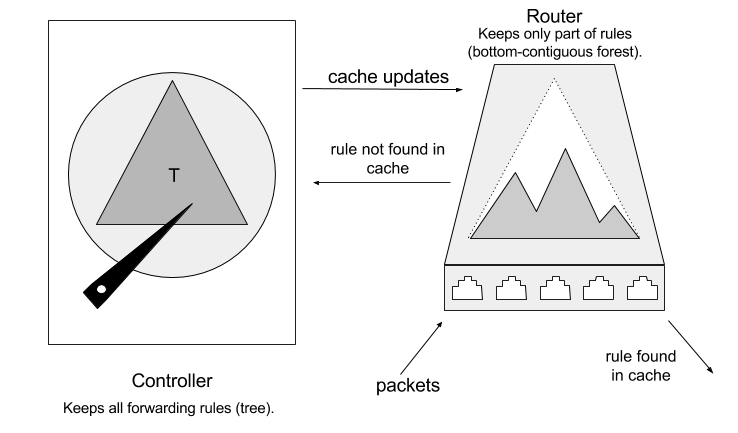
\includegraphics[width=0.8\textwidth]{motivation.png}
\end{center}
\caption{}
\label{fig:motivation}
\end{figure}

The tree caching model can be easily applied to the SND architecture 
assumptions. Fast memory here is obviously routers cache and the 
controller maps to slow memory. Positive requests correspond to looking up
forwarding rule for given packet. Whenever we want to evict an item from 
router's cache, we can send $\alpha$ negative requests in our model to trigger 
the eviction. Whats is more, the tree structure and bottom-contiguity arise 
from the FIB's longest matching prefix scheme (LMP). When we are given a 
packet, we search for forwarding rule which matches the longest prefix with the 
IP destination of packet. The IP addresses form naturally a tree like 
structure, where in the root there is the most general rule and in the leaves 
there are most precise ones. See, that if the router's cache was not 
bottom-contiguous, we would face a situation, where we would send packet to 
wrong destination finding less specific rule. This assures, that when the rule 
for packet is found in cache it is similar to the most precise rule in 
controller.
